\documentclass{beamer}
\date{\today}
\title{Multi-Agent Path Finding Visualization}
\author{Yihao Liu}

\begin{document}

\begin{frame}
  \titlepage
\end{frame}

\begin{frame}
\frametitle{Explain of Interface and Symbols}
\begin{itemize}
\item Timestamp ($h_v$): the timestamp of current step.
\item Last VNode: the VNode processed at current step.
\item $g(v)$: the Manhattan distance between the last VNode to the destination.
\item Occupied List (left): the node ($O_v$) and edge ($O_e$) constraints. \\
For node, the format is ($x$, $y$) [start, end). \\
For edge, the format is ($x$, $y$, direction) [start, end).
\item Open / Closed List (right): defined in A* algorithm. The format is ($x$, $y$) $\rightarrow$ ($x_p$, $y_p$)\quad $h_v$\quad $h_v+g(v)$, $p$ means parent.
\item Global: show all information of the nodes and edges.
\item Non global: show information of the selected node or edge.
\end{itemize}


\end{frame}

\begin{frame}
\frametitle{Initial State of Agent 1}
The circles are available nodes, they are connected by edges (lines), and the squares (or walls) are obstacles.
\begin{figure}
\centering
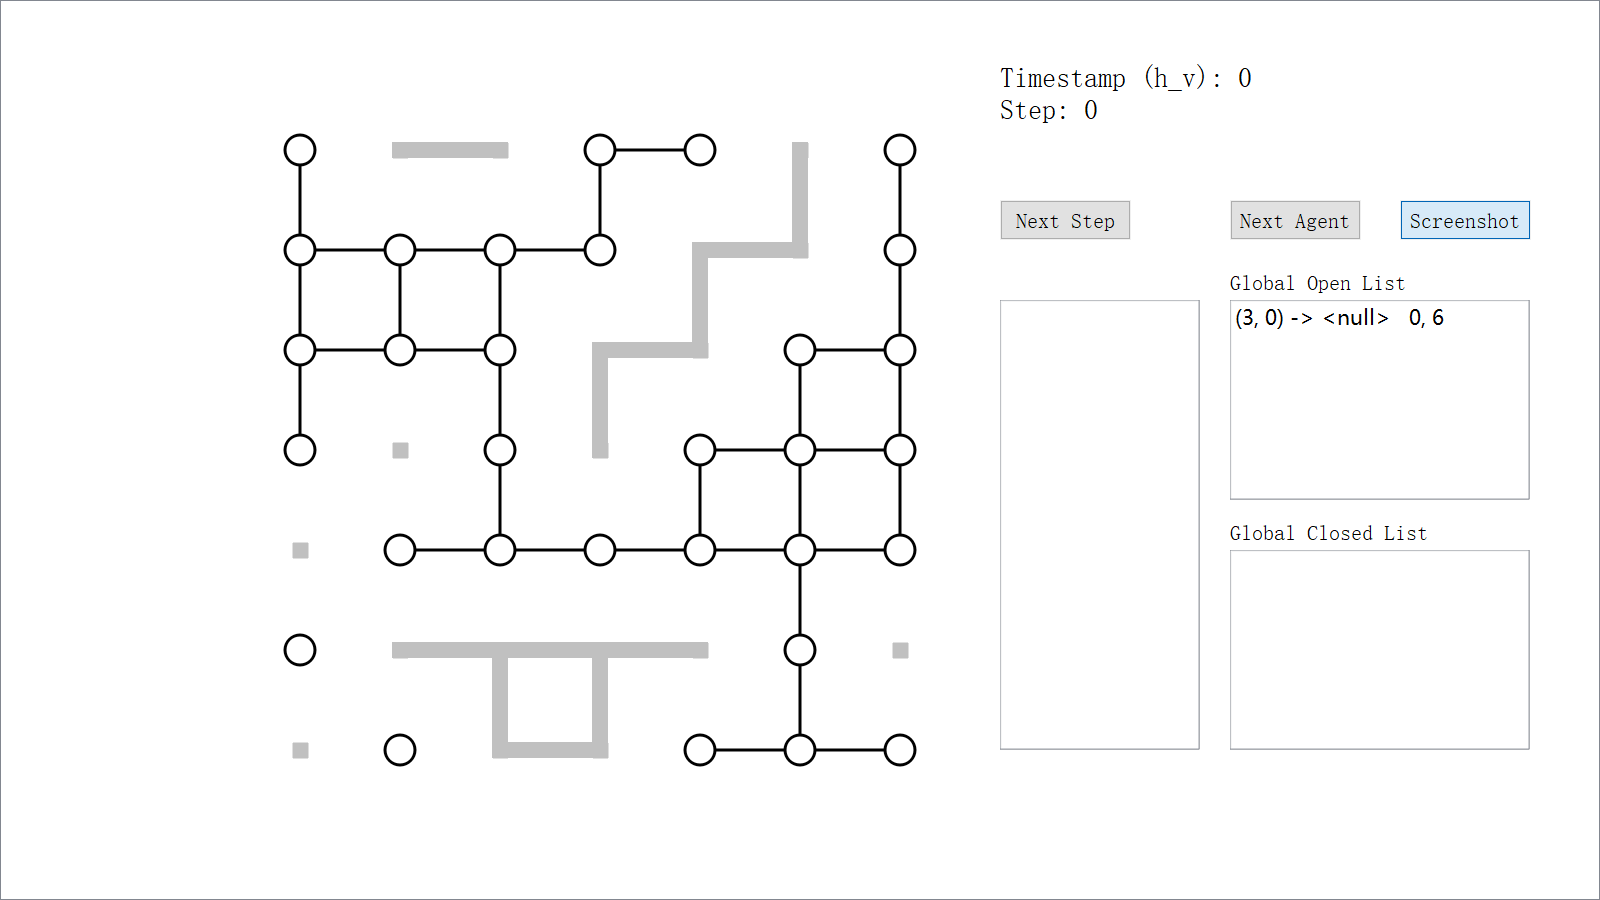
\includegraphics[width=0.8\textwidth]{a1s0.png}
\end{figure}
\end{frame}

\begin{frame}
\frametitle{First Step of Agent 1}
The location of the current agent (can also be represented by ``Last VNode'' with its position) is marked in blue with a dot inside it. 
\begin{figure}
\centering
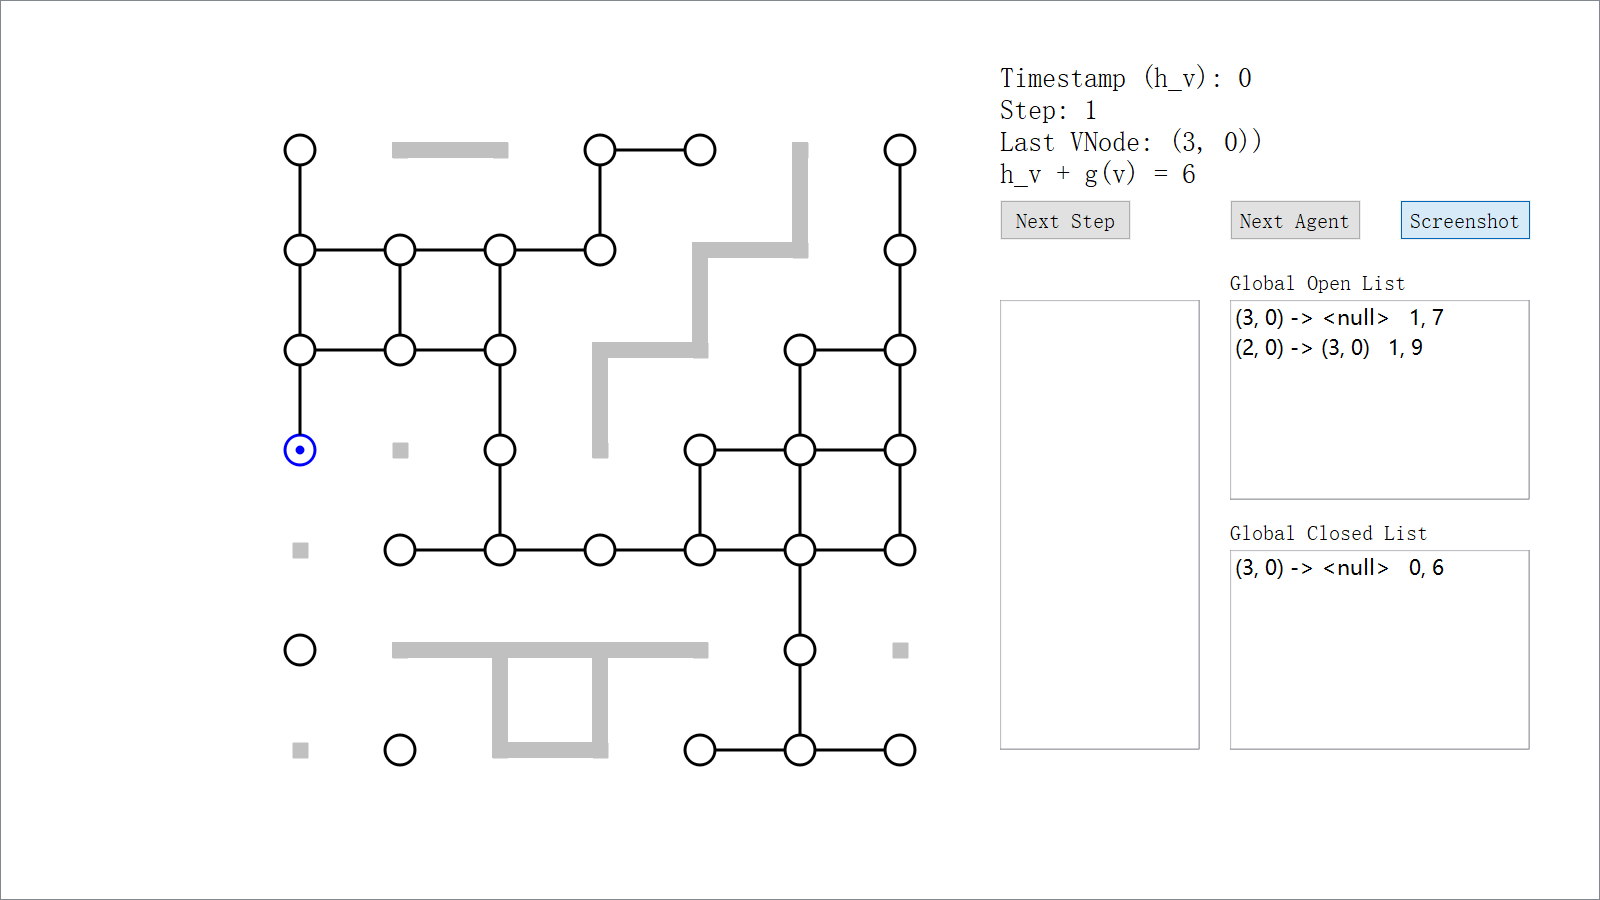
\includegraphics[width=0.8\textwidth]{a1s1.png}
\end{figure}
\end{frame}

\begin{frame}
\frametitle{Middle Step of Agent 1}
The selected node is marked in green, the open and closed list corresponding to the selected node are shown in the list in right, and the occupied status of the current node is shown in the left.
\begin{figure}
\centering
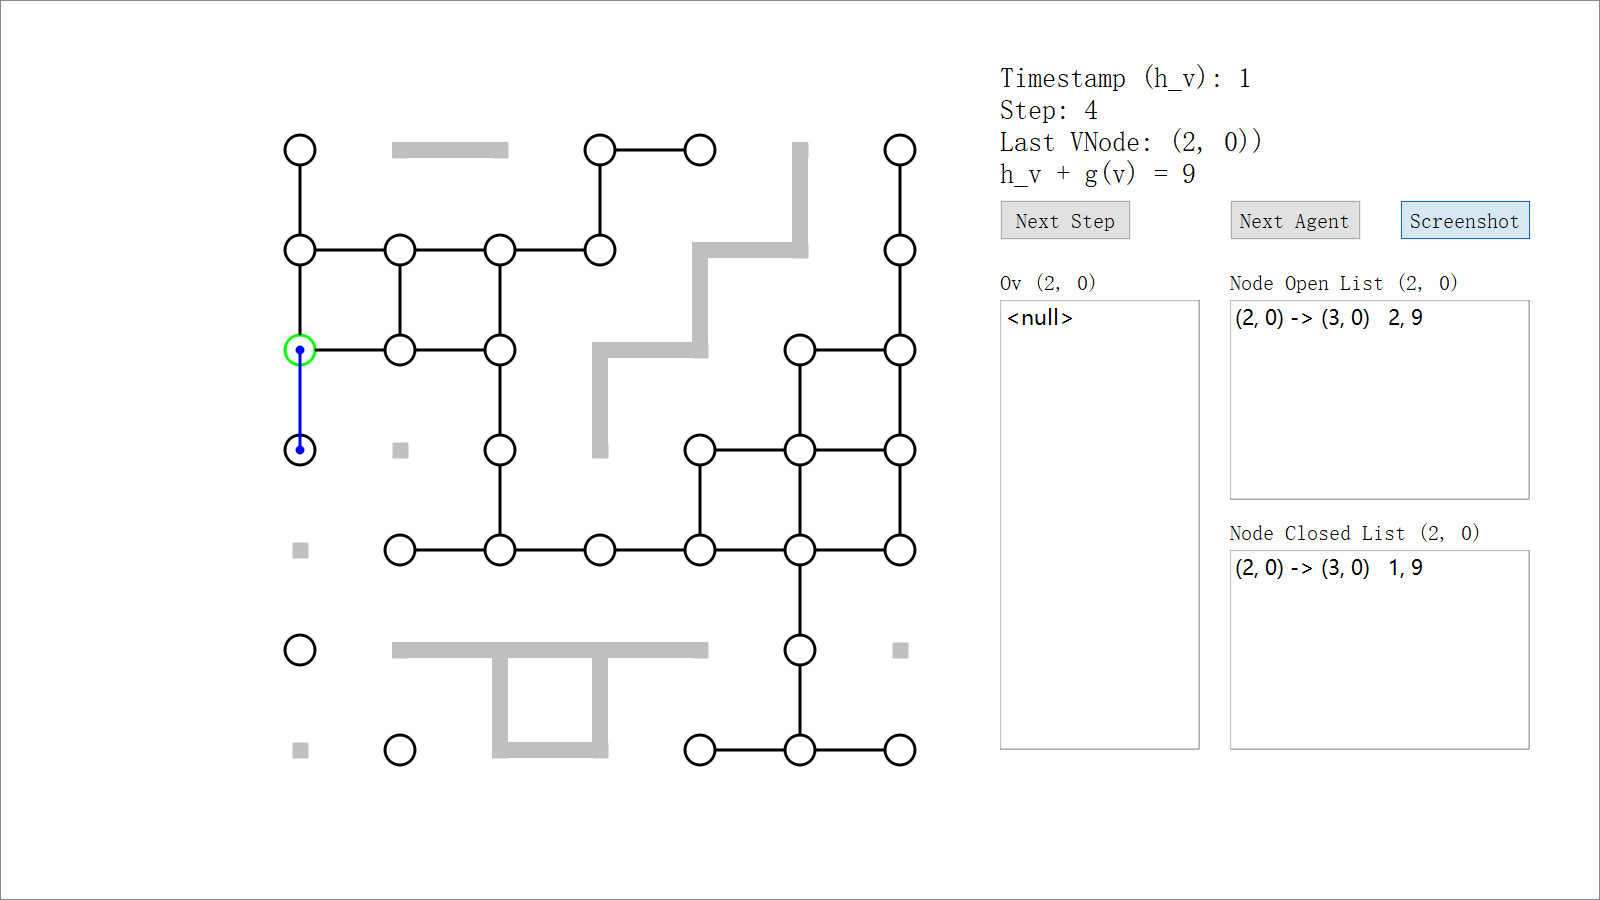
\includegraphics[width=0.8\textwidth]{a1s2.png}
\end{figure}
\end{frame}


\begin{frame}
\frametitle{Last Step of Agent 1}
The path of the current agent is also marked in blue. The open and closed list of all nodes (named ``global'') are shown in the list in right.
\begin{figure}
\centering
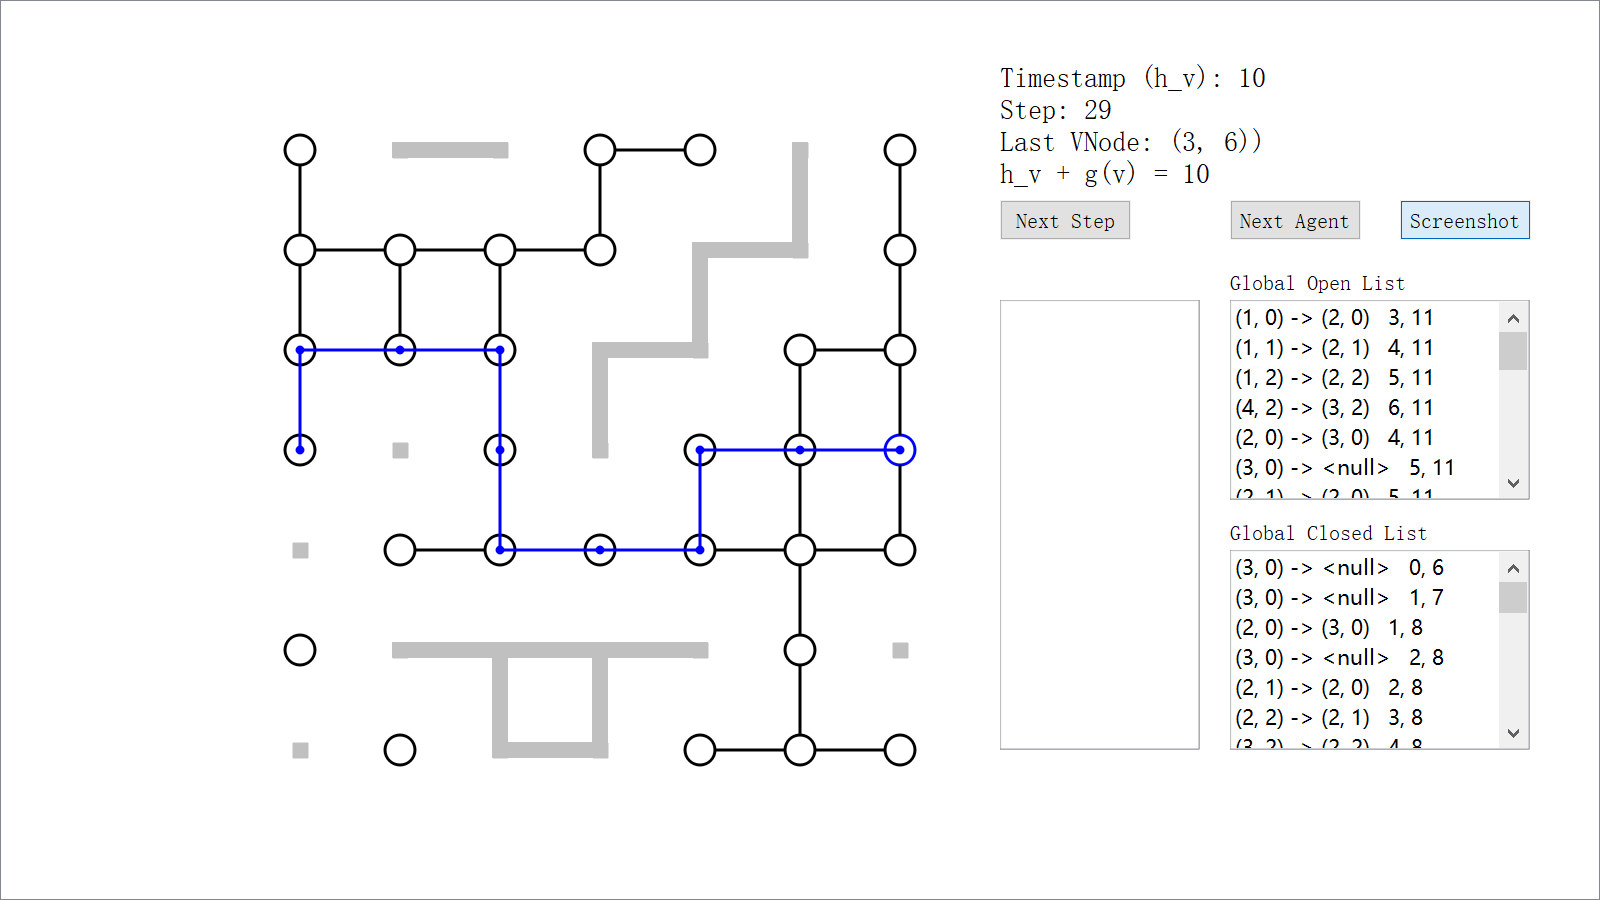
\includegraphics[width=0.8\textwidth]{a1s3.png}
\end{figure}
\end{frame}

\begin{frame}
\frametitle{Initial State of Agent 2}
The constraints at the current timestamp are marked in red. At timestamp 0, they are the starting node and first edge of Agent 1.
\begin{figure}
\centering
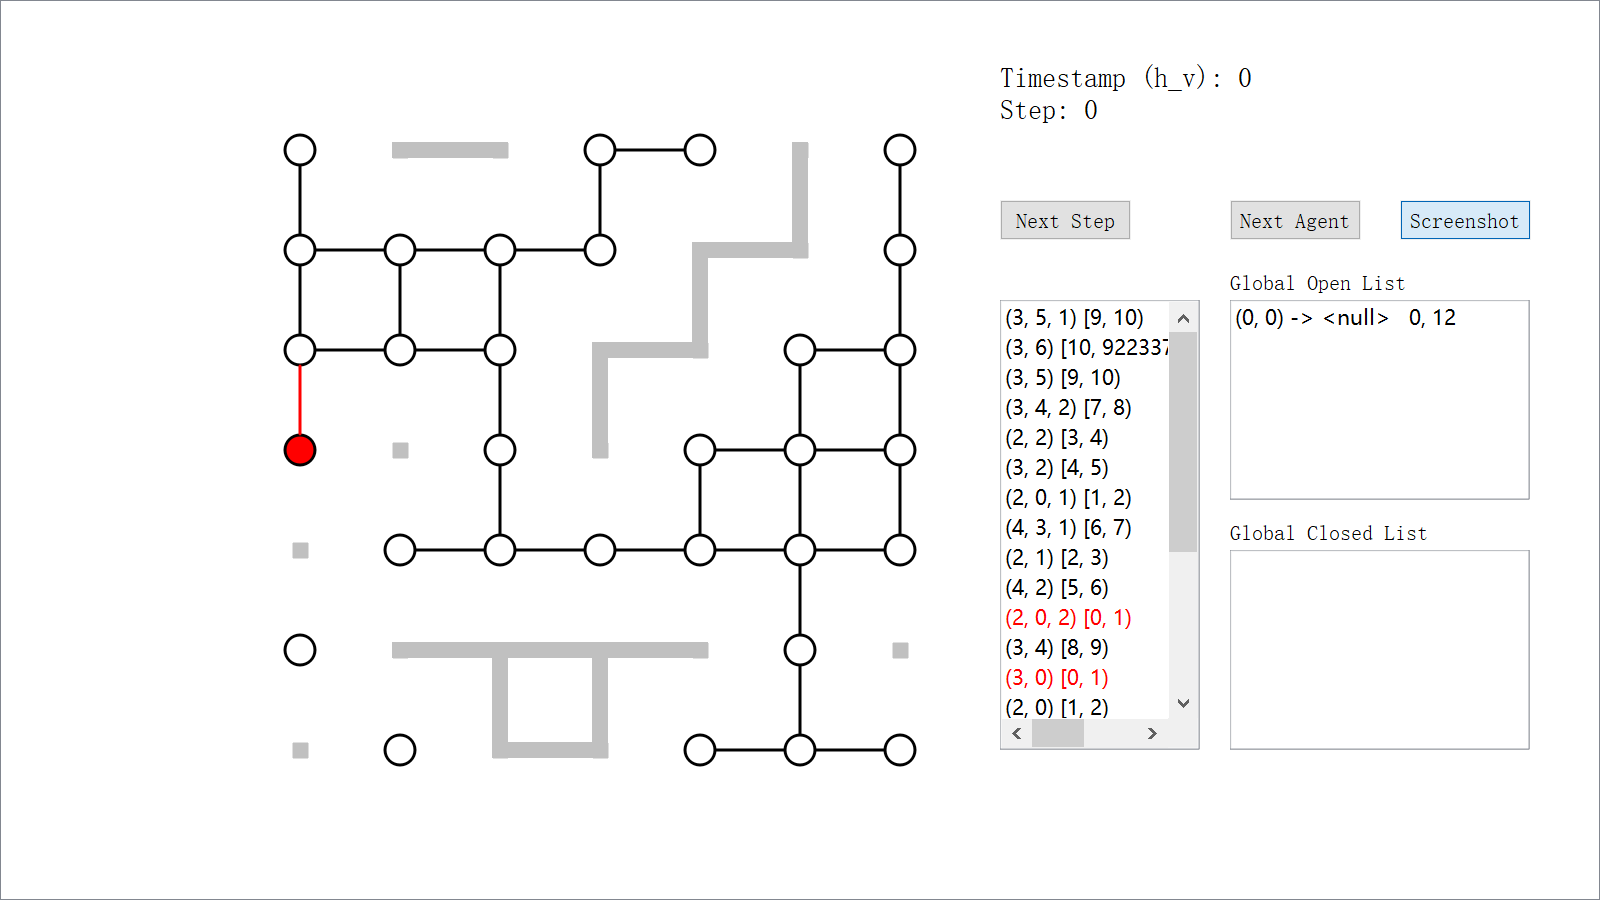
\includegraphics[width=0.8\textwidth]{a2s0.png}
\end{figure}
\end{frame}

\begin{frame}
\frametitle{First Step of Agent 2}
$h_v$ is the current timestamp, $g(v)$ means the Manhattan distance between the last VNode to the destination, so $h_v+g(v)$ is an lower bound estimate of the arrival time of the agent at that VNode.
\begin{figure}
\centering
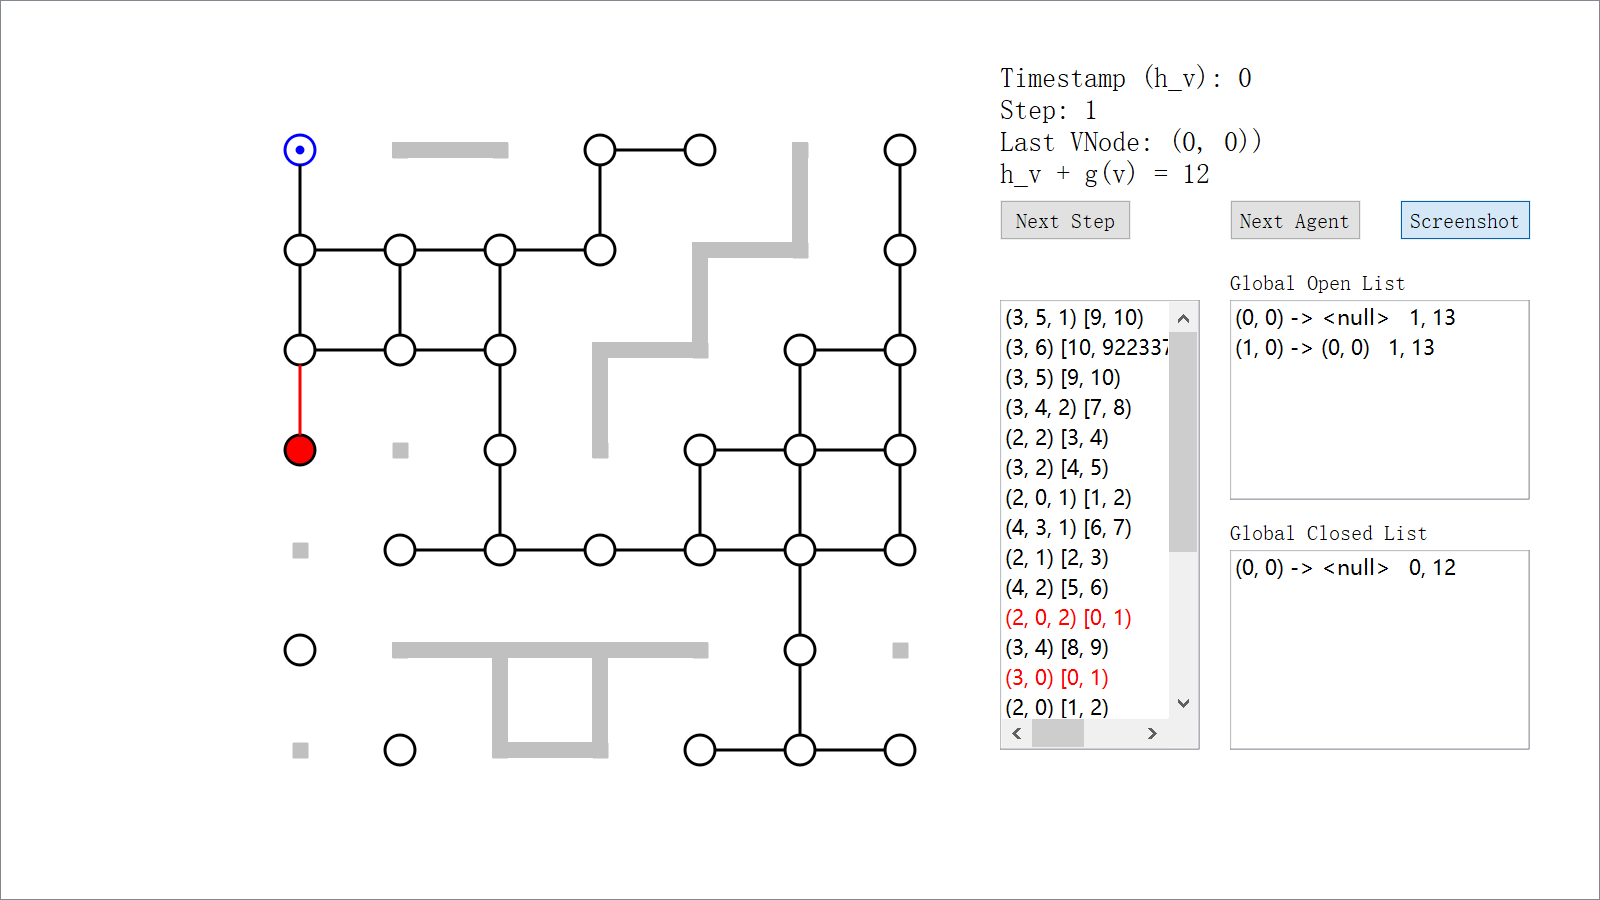
\includegraphics[width=0.8\textwidth]{a2s1.png}
\end{figure}
\end{frame}

\begin{frame}
\frametitle{Middle Step of Agent 2}
After some time the current constraints may change. Note that in the list in left all constraints are listed, in which red means that it's effective currently, and the tuple represents (x, y, direction) for edge constraint, or (x, y) for node constraint.
\begin{figure}
\centering
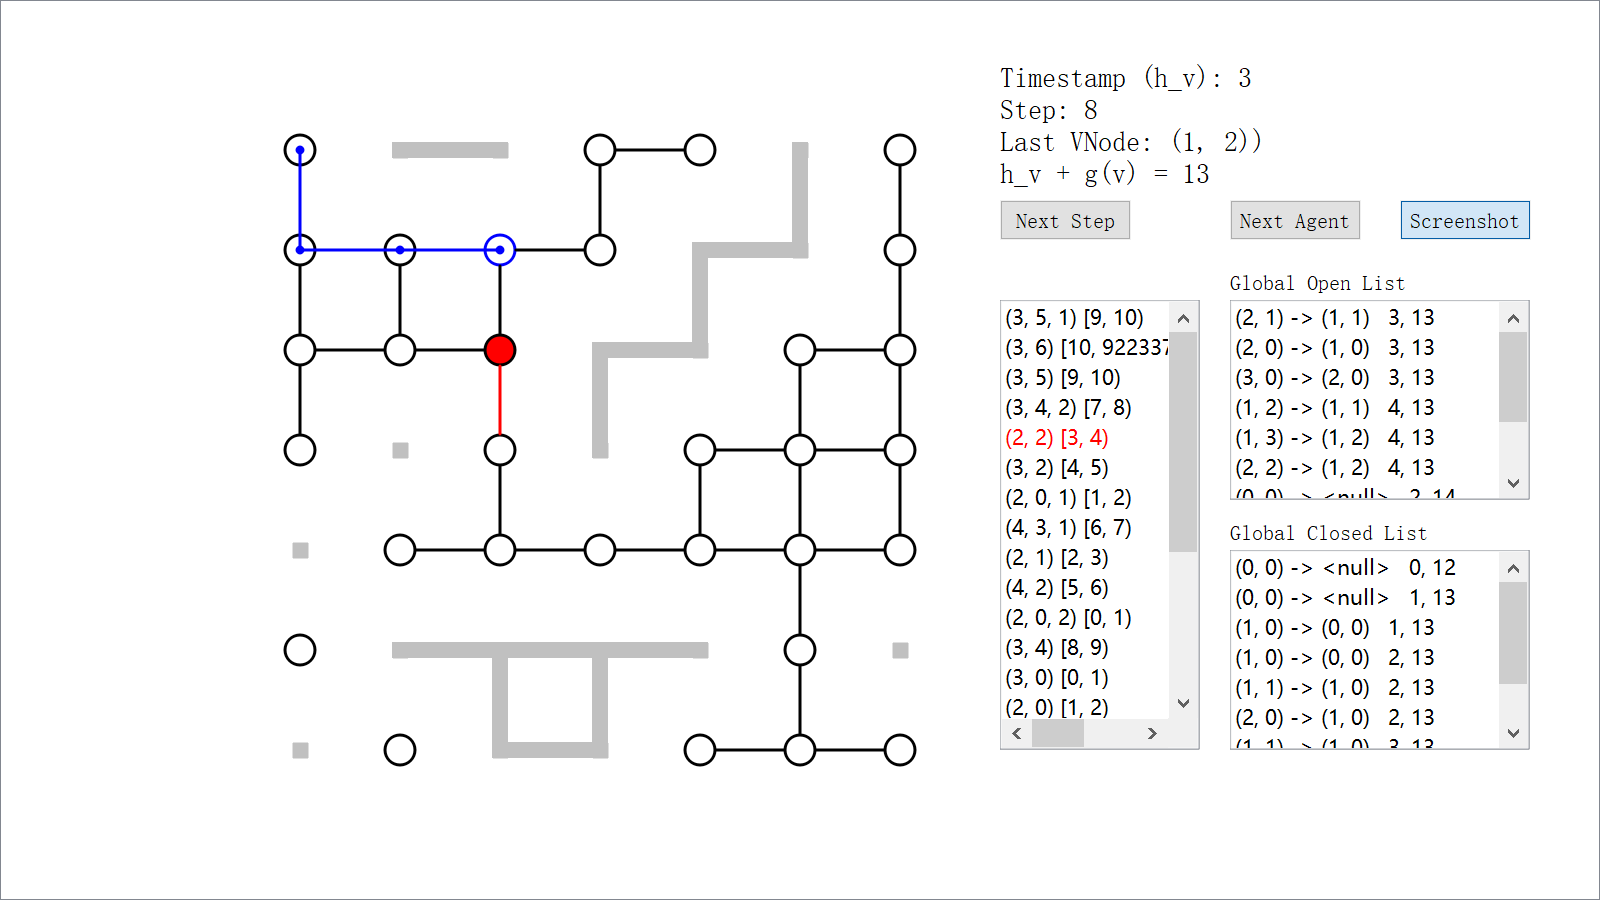
\includegraphics[width=0.8\textwidth]{a2s2.png}
\end{figure}
\end{frame}

\begin{frame}
\frametitle{Last Step of Agent 2}
The arrow ($\rightarrow$) in the open and closed list represents a parent (right) relation of a VNode (left). Then the path can be constructed reversely according to these relations beginning with the VNode at the destination.
\begin{figure}
\centering
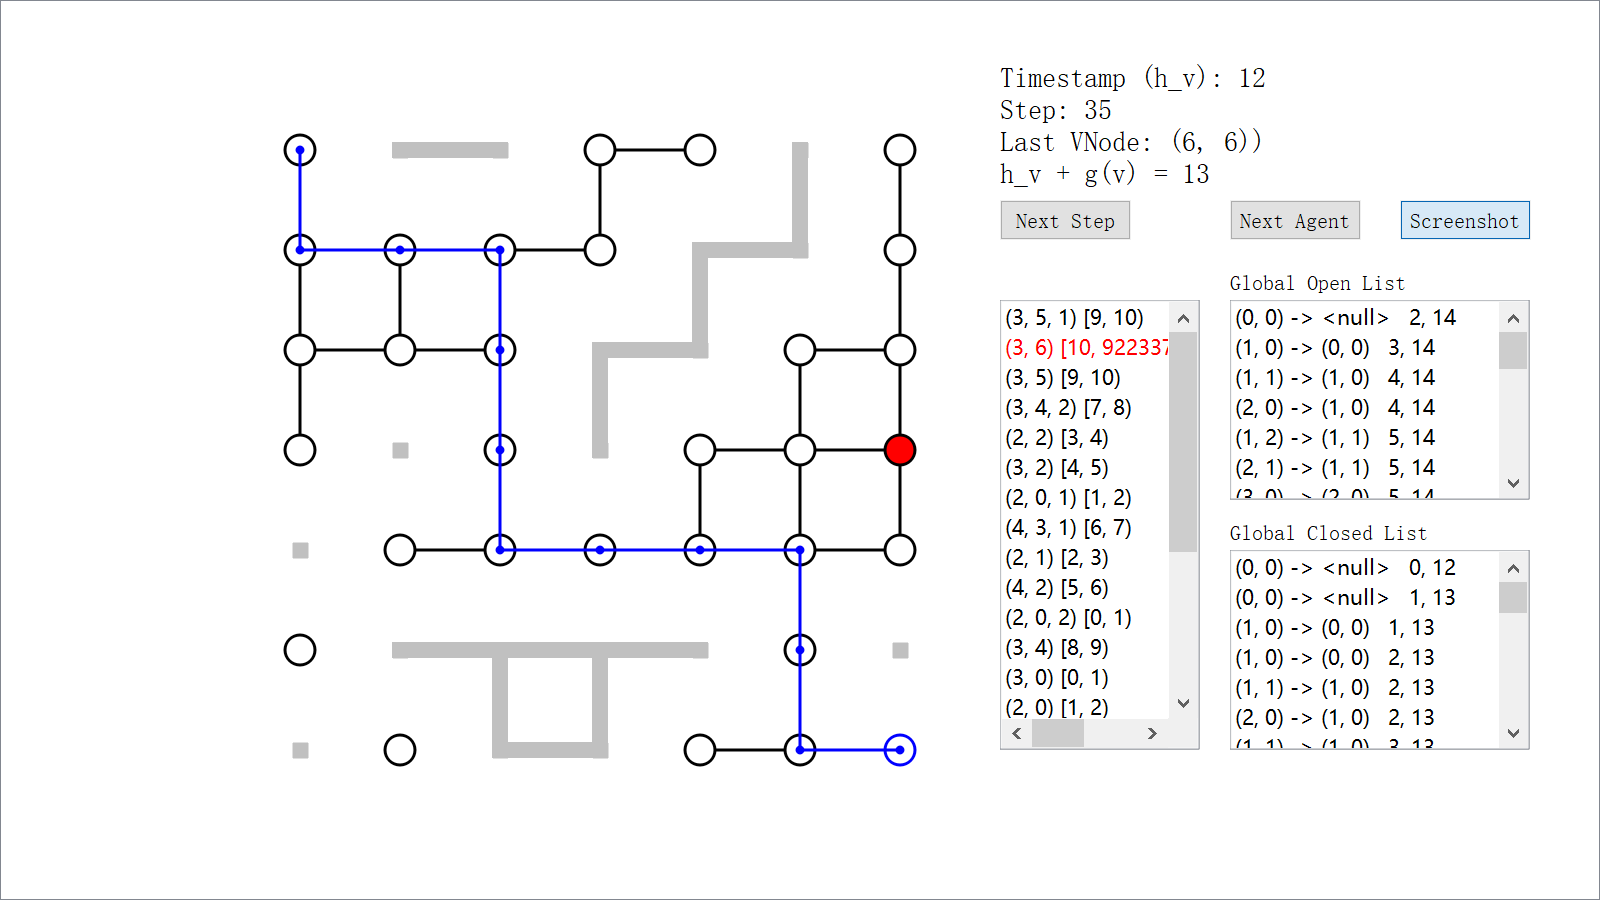
\includegraphics[width=0.8\textwidth]{a2s3.png}
\end{figure}
\end{frame}

\end{document}

